\section{Use cases identification}
\subsection{Scenarios}
Here are some scenarios that describe the usage of the system.
\subsubsection{Scenario 1}
\label{scenario:1}
Francesco wants to have a beer with his friend Vincenzo so Francesco logs in to system and searches for cars nearby. He notices that there are two cars available next to his house, he decides to reserve the one with more battery and after few minutes he reaches it. He starts to drive until he reaches Vincenzo's house, Vincenzo gets into the car and they arrive to the beer house where they terminate the rent.

\subsubsection{Scenario 2}
\label{scenario:2}
Mirjana has been told by her friend Elisa that a new car sharing service is available in their city and so she decided to give it a try as she wants to go shopping in the city center. She registers to the system providing all information requested, she inserts the destination address and enables the money saving option. She is provided by the system with a charging station not far from the shopping center and, as it is a sunny day, she decided to take that location as destination in order to achieve a discount and reach the shopping center on foot. 

\subsubsection{Scenario 3}
\label{scenario:3}
Giovanni is really interested in electric cars so he decides to use the PowerEnJoy system. He wants to go to the museum in the afternoon so he reserves a car. After one hour he is \todo{is he notified?}notified by the system that his reservation is expired and he is charged of a 1\euro\ fee. When he is ready to exit his house he notices that the same car is still available so he reserves it again, reaches it and starts driving. When he arrives at the destination he sees a charging station next to the museum so he decides to leave the car there plugging the charging cable in order to get a discount.

\subsubsection{Scenario 4}
\label{scenario:4}
Dino reserves a car, he reaches it and unlock the doors. He starts driving but after few minutes the engine stops and a warning icon lights up in the dashboard. He contacts the customer care service that suggests him to reserve a different car which is nearby, the customer care operator then tags the first car as not available specifying a brief description of the fault. The maintenance service is now aware of the problem and they take care of resolving the issue: a maintenance operator is sent to the car, he unlock it \todo{how he unlocks the car?} and fix it. When the car is fully functional he tags it as available using a restricted access API of our system.
\clearpage
\subsection{Use case diagram}
%\begin{center}
%  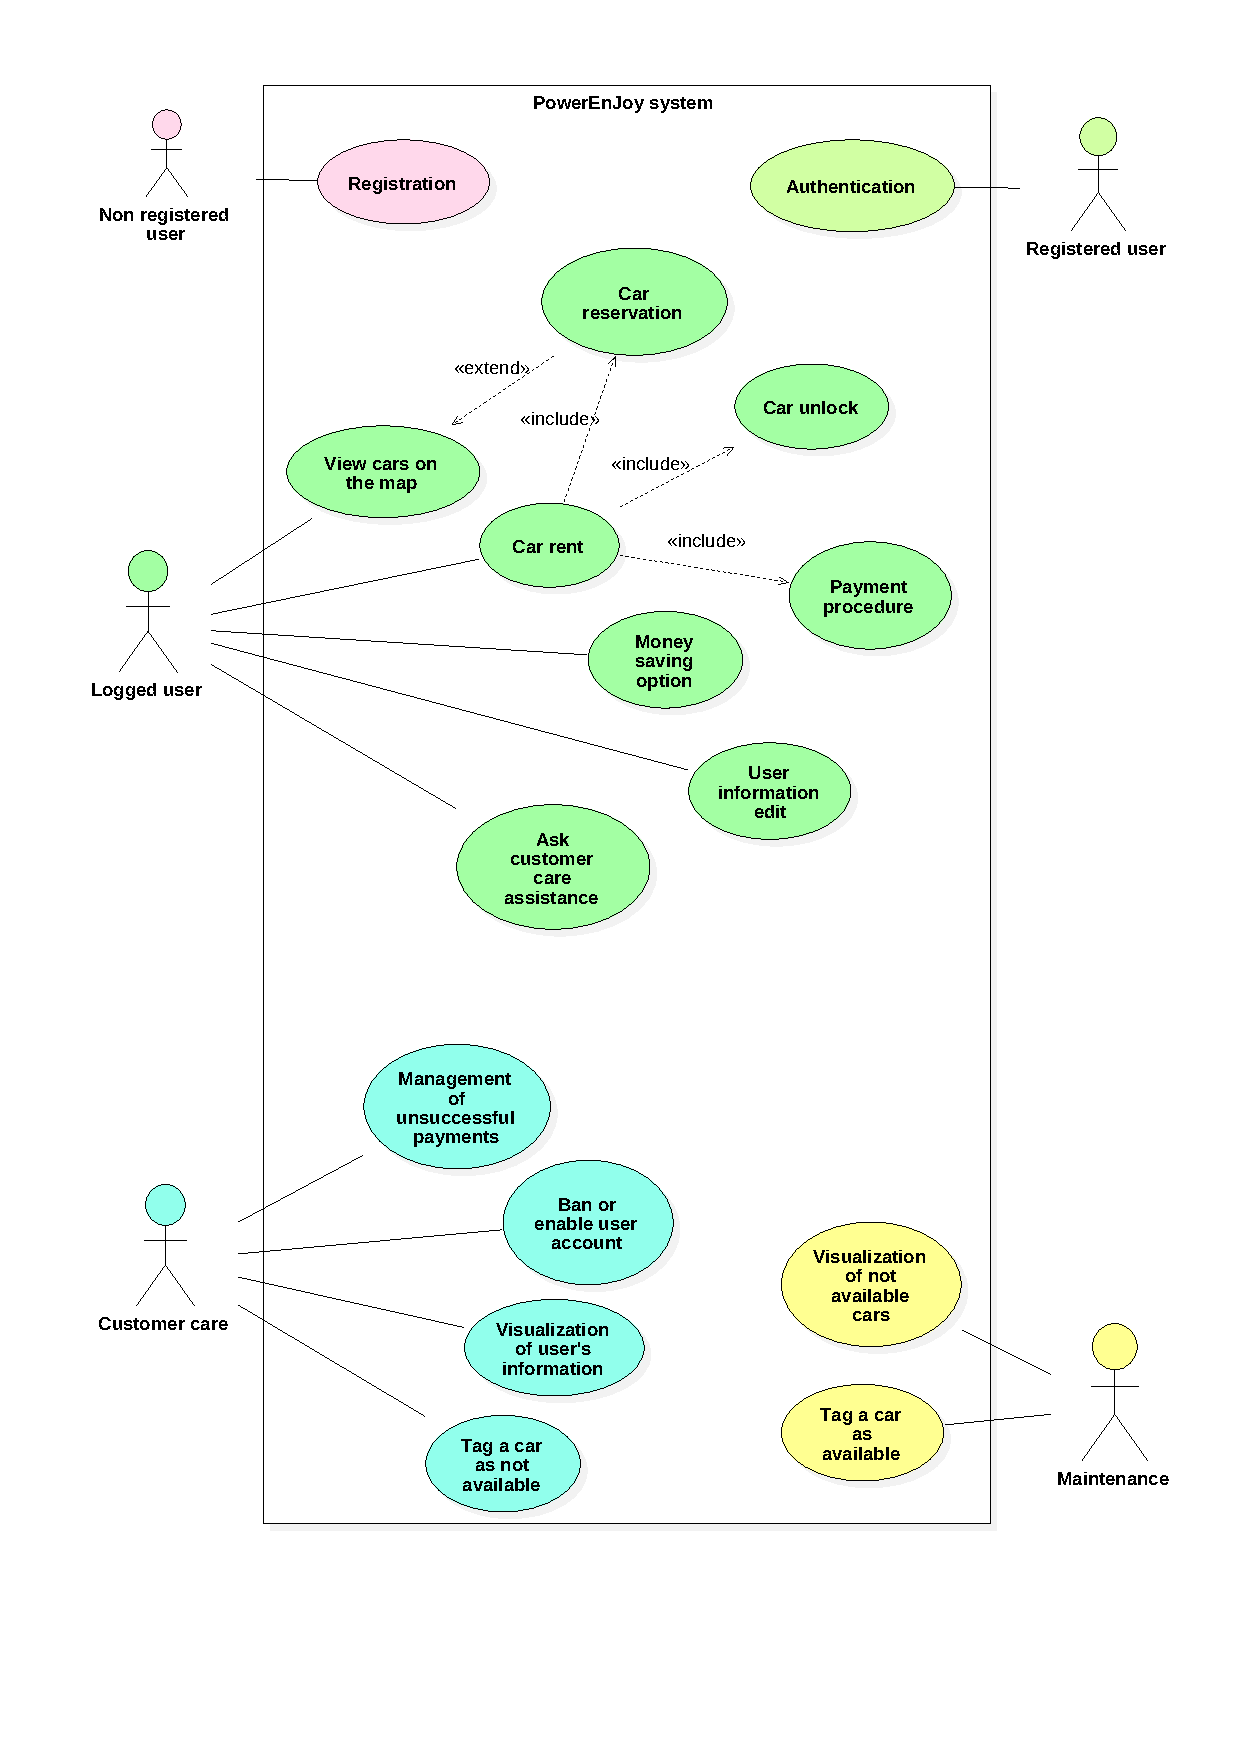
\includegraphics[width=0.9\textwidth]{useCase}
%  \captionof{figure}{Use case diagram}
%  \label{fig:useCase}
%\end{center}

\begin{figure}[h!]
	\centering
	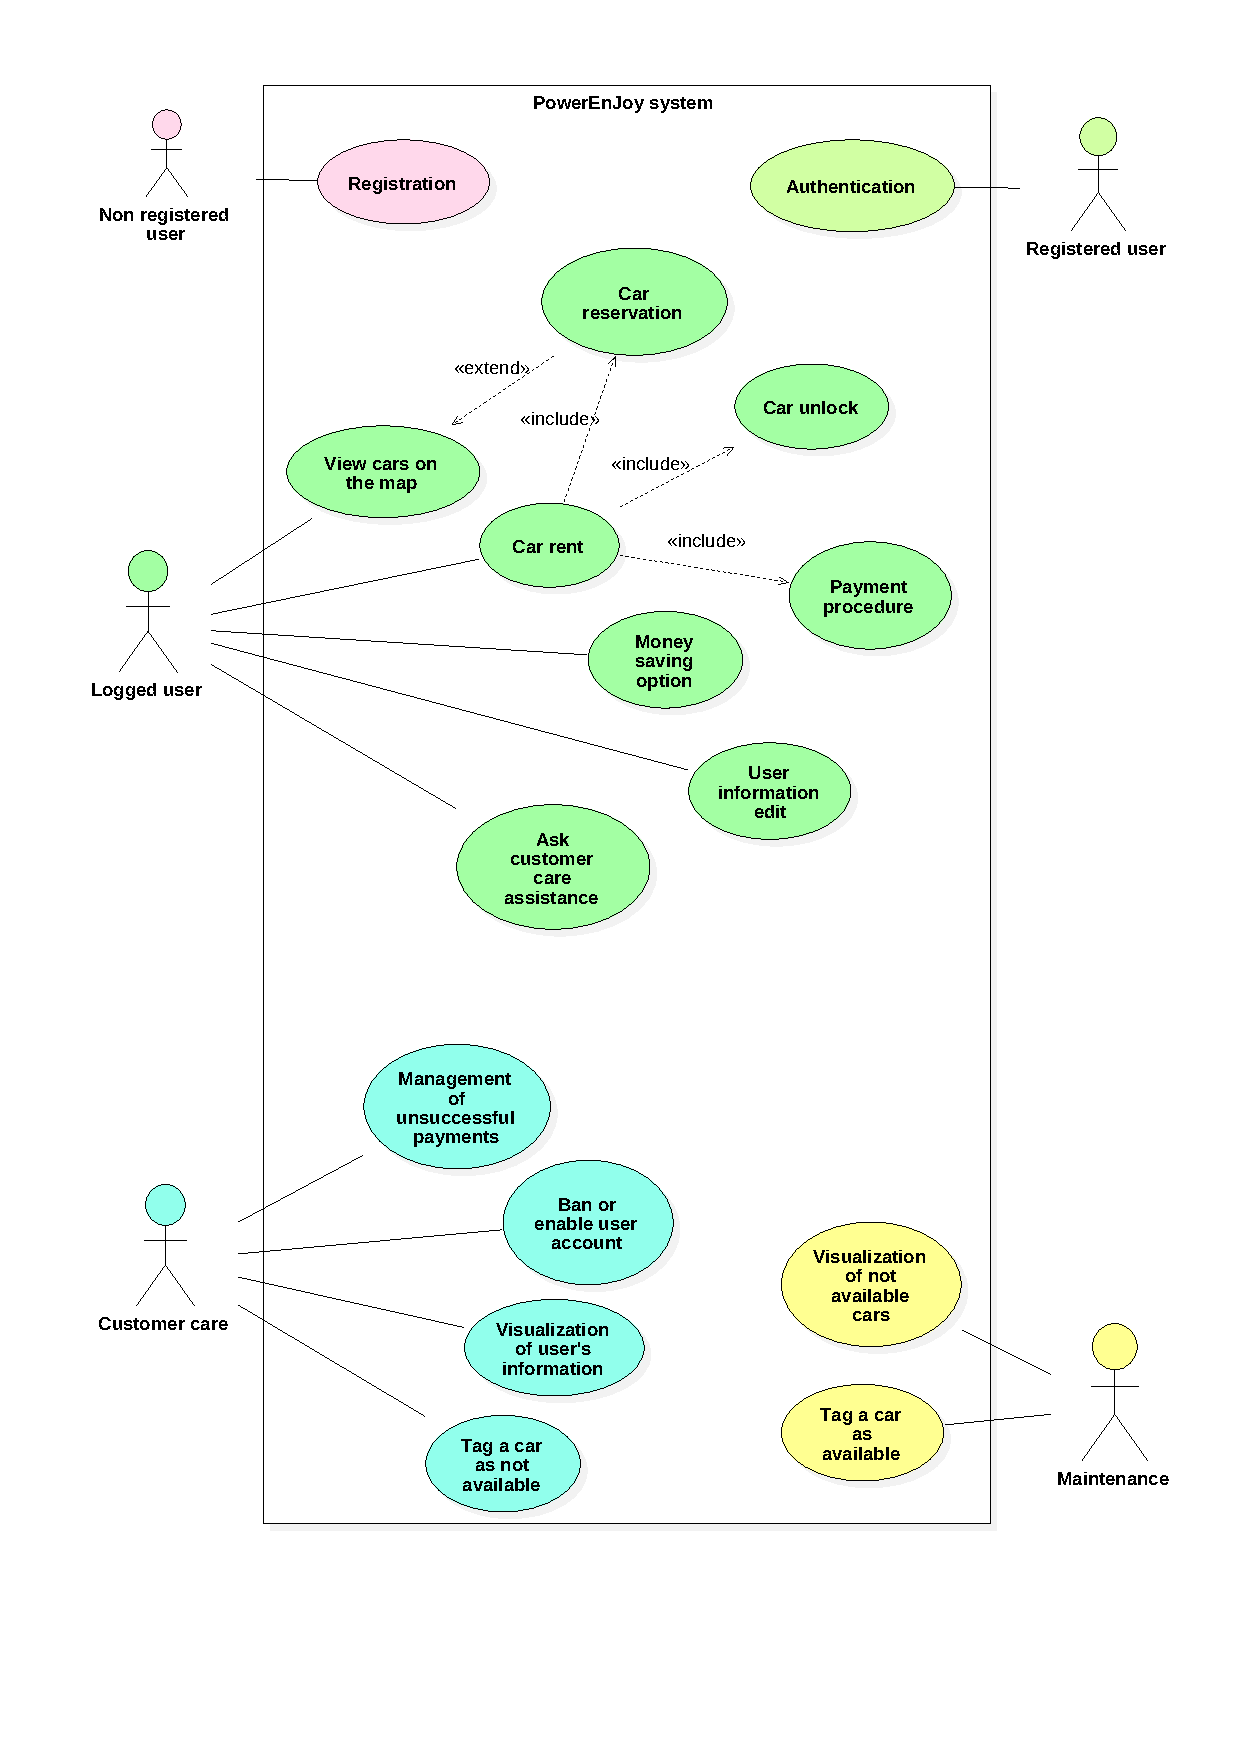
\includegraphics[width=\linewidth]{useCase}
	\caption{
		\label{fig:useCase} 
		Use case diagram
	}
\end{figure}
\clearpage

\subsection{Use cases description}
\subsubsection{Registration}
\begin{longtable}{p{0.25\linewidth}p{0.75\linewidth}}
\toprule
\textbf{Name} & \textbf{Registration} \\
\midrule
\textbf{Actors} & Non registered user \\
\midrule
\textbf{Entry conditions} & \\
\midrule
\textbf{Flow of events} & 
\begin{enumerate}
	\item The user asks the system to register to its services
	\item The system shows the appropriate form to fill to register to the system
	\item The user inserts an username to be uniquely identified by the system
	\item The user inserts his own email address
	\item The user inserts his name, surname, birth date and place and current domicile
	\item The user inserts his driving license ID code and expiring date
	\item The user inserts payment information
	\item The user confirms data inserted are correct e submit the form
	\item The system sends an email to the user with a unique link to verify the email address inserted by the user really belongs to him
	\item The user clicking on the link received confirms his email address
	\item The user is notified by mail the registration procedure is correctly completed
\end{enumerate} \\
\midrule
\textbf{Exit conditions} & The user is provided with a password bound to his username to access the system\\
\midrule
\textbf{Exceptions} & 
\begin{itemize}
	\item If the username inserted by the user is already used by another user, the system displays an error message asking the user to insert another username
	\item If the user doesn't receive the link sent to him by mail needs to complete the form again with a correct email address
	\item If the user notices to have entered wrong informations he could edit them at the end of the process of registration in his personal page
\end{itemize} \\
\bottomrule
\caption{\emph{Registration} use case description}
\end{longtable}

\begin{figure}[h!]
	\centering
	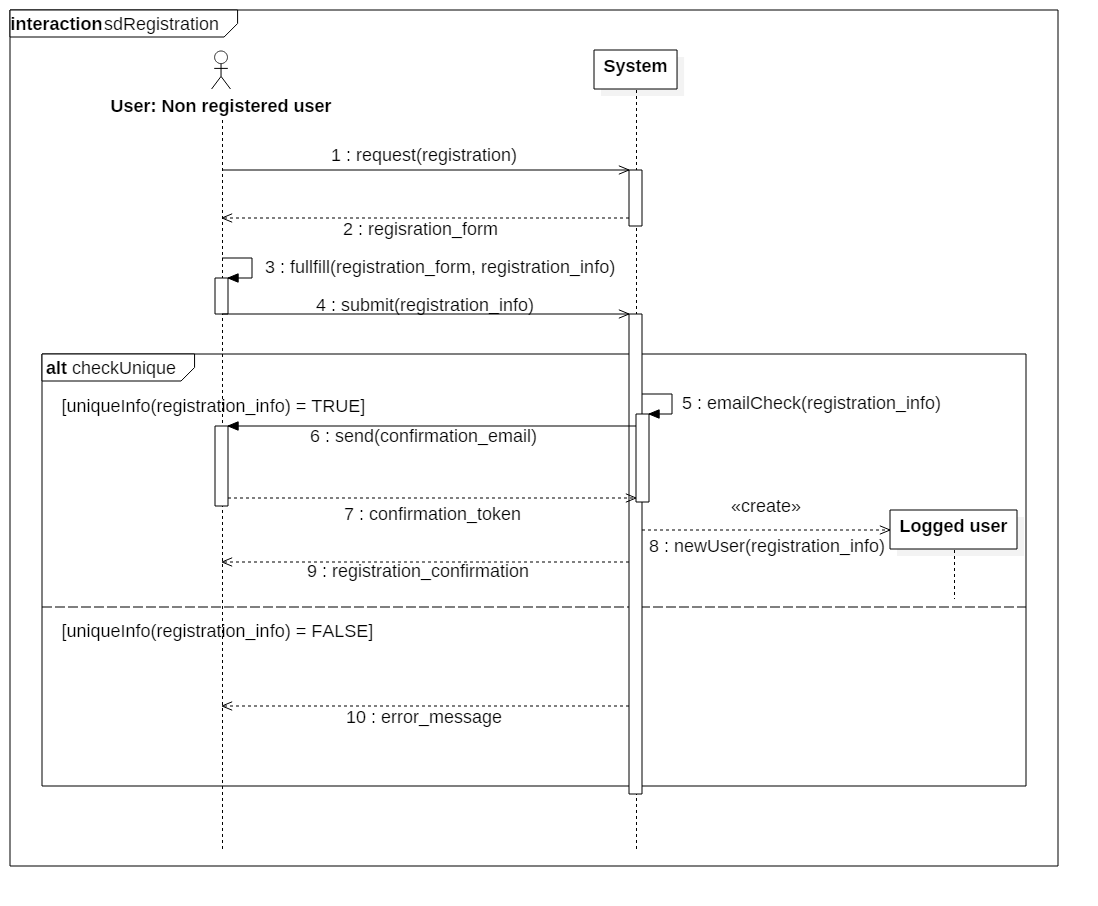
\includegraphics [width=\textwidth]{/diagrams/Sequence/sdRegistration.png}
	\caption{
		\label{fig:registrationSequence} 
		Registration sequence diagram
	}
\end{figure}

%///////////////////////////////////////////////////////////
\clearpage
\subsubsection{Authentication}
\begin{longtable}{p{0.25\linewidth}p{0.75\linewidth}}
\toprule
\textbf{Name} & \textbf{Authentication} \\
\midrule
\textbf{Actors} &  Registered user \\
\midrule
\textbf{Entry conditions} & The user must know his username and password \\
\midrule
\textbf{Flow of events} & 
\begin{enumerate}
	\item The user inserts his username and password in the appropriate form and submit it
	\item The system validates the inserted credential
	\item The system checks if the user is banned
\end{enumerate} \\
\midrule
\textbf{Exit conditions} & If the credential validation is successful and the user is not banned he is granted the proper privileges\\
\midrule
\textbf{Exceptions} & 
\begin{itemize}
	\item If the credential validation failed an error message is displayed
	\item If the credential validation is successful and the user is banned a message providing assistance is displayed and the system doesn't allows the user to access to the system
\end{itemize} \\
\bottomrule
\caption{\emph{Authentication} use case description}
\end{longtable}


\begin{figure}[h!]
	\centering
	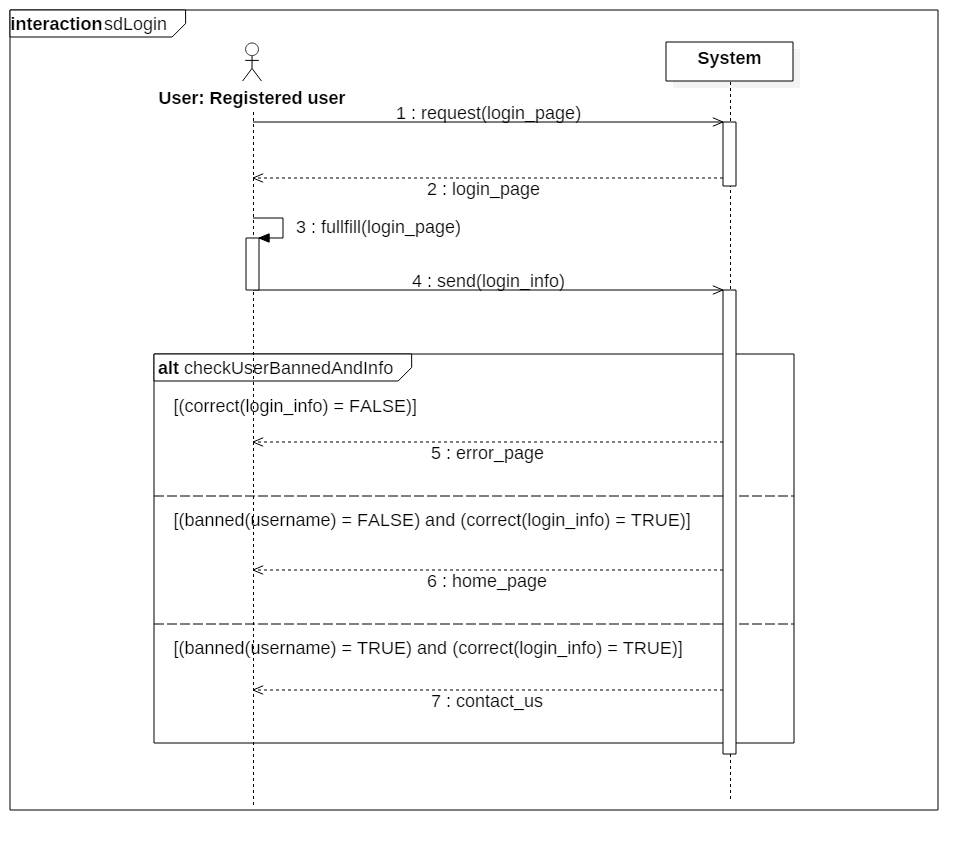
\includegraphics [width=\textwidth]{/diagrams/Sequence/sdLogin.png}
	\caption{
		\label{fig:authSequence} 
		Authentication sequence diagram
	}
\end{figure}

%///////////////////////////////////////////////////////////
\clearpage
\subsubsection{View cars on the map}
\begin{longtable}{p{0.25\linewidth}p{0.75\linewidth}}
\toprule
\textbf{Name} & \textbf{View cars on the map} \\
\midrule
\textbf{Actors} &  Logged user \\
\midrule
\textbf{Entry conditions} & \\
\midrule
\textbf{Flow of events} & 
\begin{enumerate}
	\item The user chooses if he wants to use his GPS position or insert a different one manually
		\subitem a. The system retrieves the user's GPS position
		\subitem b. The user inserts a position
	\item The system retrieves the position of all available cars and their battery level percentage
	\item The system shows a map with all available cars near the position indicated by the user
	\item The user can click on a car on the map to see its battery level percentage
\end{enumerate}\\
\midrule
\textbf{Exit conditions} & The user can navigate a map with all available cars near the position indicated by him\\
\midrule
\textbf{Exceptions} & 
If the position inserted by the user is not correct an error message is displayed \\
\bottomrule
\caption{\emph{View cars on the map} use case description}
\end{longtable}

%///////////////////////////////////////////////////////////
\clearpage
\subsubsection{Car reservation}
\begin{longtable}{p{0.25\linewidth}p{0.75\linewidth}}
\toprule
\textbf{Name} & \textbf{Car reservation} \\
\midrule
\textbf{Actors} &  Logged user \\
\midrule
\textbf{Entry conditions} & \\
\midrule
\textbf{Flow of events} & 
\begin{enumerate}
	\item \textbf{View cars on the map}
	\item The user selects the car he wants to reserve
	\item The user confirms he wants to reserve that car
\end{enumerate}\\
\midrule
\textbf{Exit conditions} & The system set the state of the chosen car as \emph{Reserved} paired with the user who made the reservation\\
\midrule
\textbf{Exceptions} &  If the user has already reserved a car, the system shows an error message and doesn't allow him to reserve another car \\
\bottomrule
\caption{\emph{Car reservation} use case description}
\end{longtable}


\begin{figure}[h!]
	\centering
	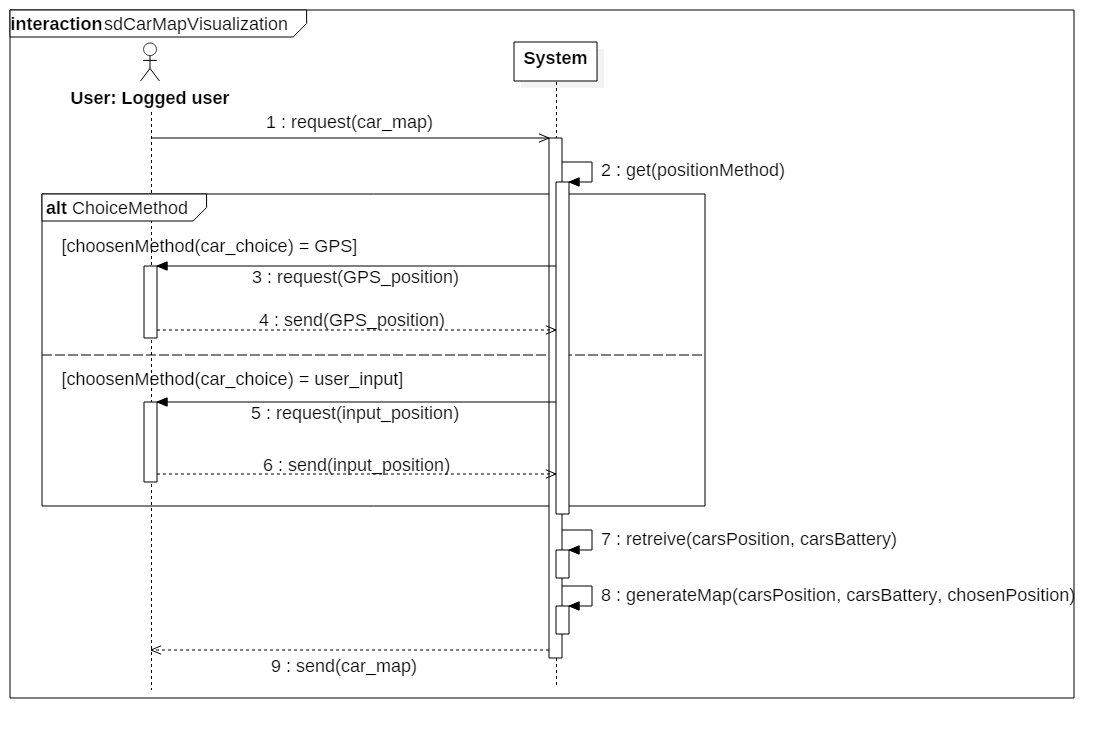
\includegraphics [width=\textwidth]{/diagrams/Sequence/sdCarMapVisualization.png}
	\caption{
		\label{fig:carsMapSequence} 
		View cars on the map sequence diagram
	}
\end{figure}

%///////////////////////////////////////////////////////////
\clearpage
\subsubsection{Car unlock}
\begin{longtable}{p{0.25\linewidth}p{0.75\linewidth}}
\toprule
\textbf{Name} & \textbf{Car unlock} \\
\midrule
\textbf{Actors} &  Logged user \\
\midrule
\textbf{Entry conditions} & The user reserved car \\
\midrule
\textbf{Flow of events} & 
\begin{enumerate}
	\item The user asks the system to unlock the car he reserved
	\item The system checks if the user's position is at most 5 meters away from the position of the car he reserved
	\item The system unlocks the car
	\item The system sends a message to the user, confirming that the car is unlocked
\end{enumerate} \\
\midrule
\textbf{Exit conditions} & The car is unlocked and the user can pick it up\\
\midrule
\textbf{Exceptions} & 
\begin{itemize}
	\item If the position of the user is not at most 5 meters away from the position of the car he reserved the system displays an error message
\end{itemize} \\
\bottomrule
\caption{\emph{Car unlock} use case description}
\end{longtable}


\begin{figure}[h!]
	\centering
	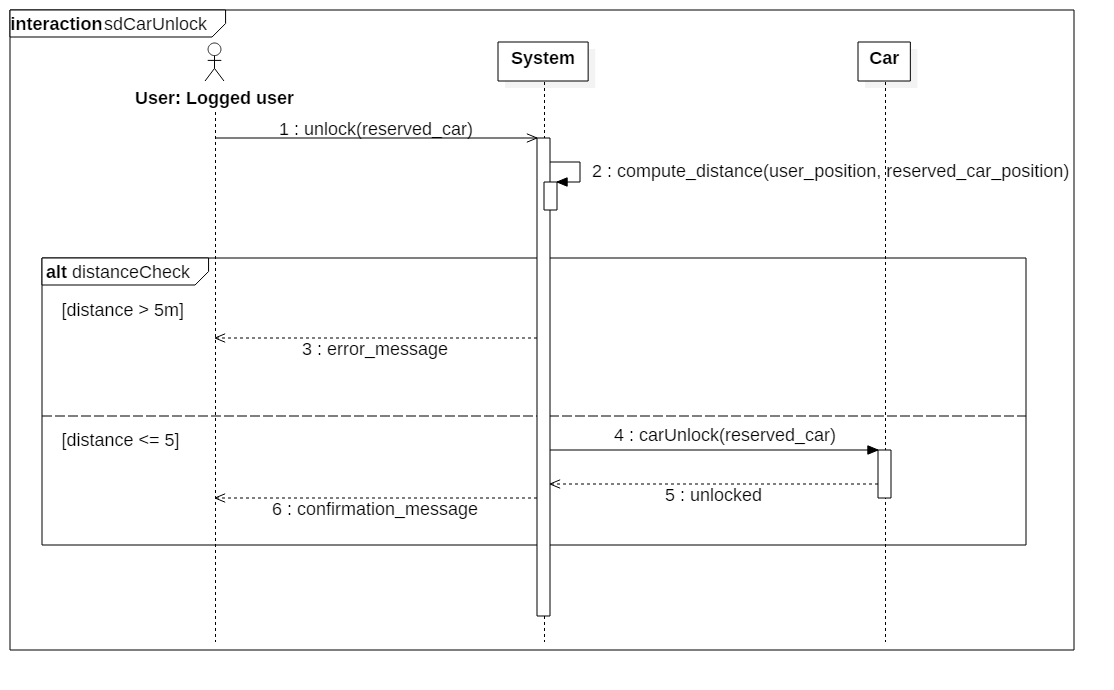
\includegraphics [width=\textwidth]{/diagrams/Sequence/sdCarUnlock.png}
	\caption{
		\label{fig:carUnlockSequence} 
		Car unlock sequence diagram
	}
\end{figure}

%///////////////////////////////////////////////////////////
\clearpage
\subsubsection{Car rent}
\begin{longtable}{p{0.25\linewidth}p{0.75\linewidth}}
\toprule
\textbf{Name} & \textbf{Car rent} \\
\midrule
\textbf{Actors} &  Logged user \\
\midrule
\textbf{Entry conditions} & 
The user is paired with the \emph{Reserved} state of a car\\
\midrule
\textbf{Flow of events} & 
\begin{enumerate}
	\item \textbf{Car unlock}
	\item The user ignites the car engine
	\item The system sets the state of the \emph{Reserved} car to \emph{In Use} paired
	with the same user
	\item During the rent the user is informed about the current charge and whether he is or not inside a safe area
	\item The user leaves the auto turning off the engine
	\item The system locks the car
    \item The system activates a timer to allow the user to plug the car into a power grid if it is
    near one of them
	\item When the timer expires: \textbf{Rent payment}
	\item The system sets the car as \emph{Available}
\end{enumerate} \\
\midrule
\textbf{Exit conditions} & 
The user is charged of the correct amount for the ride and at anytime could perform another rent, the car is available again\\
\midrule
\textbf{Exceptions} & 
\begin{itemize}
	\item If the user doesn't start the engine up to one hour after the reservation, he is charged of 1\euro , the car state is set as \emph{Available} and the user is notified his reservation is expired
\end{itemize} \\
\bottomrule
\caption{\emph{Car rent} use case description}
\end{longtable}

%///////////////////////////////////////////////////////////
\clearpage
\subsubsection{Rent payment}
\begin{longtable}{p{0.25\linewidth}p{0.75\linewidth}}
\toprule
\textbf{Name} & \textbf{Rent payment} \\
\midrule
\textbf{Actors} &  Logged user\\
\midrule
\textbf{Entry conditions} & 
The user must have completed a rent shutting off the engine and exiting the car. The timer activated by the system locking the car expires. \\
\midrule
\textbf{Flow of events} & 
\begin{enumerate}
	\item The system checks if the car position is or is not inside a safe area
	\item The system checks if the car has detected more then one passenger during the rent
	\item The system checks the car battery percentage
	\item The system checks if the car is plugged on a charging station
	\item The system checks the distance of the car from the nearest charging station
	\item The system calculates the cost of the ride based on the rent time
	\item The system determines the applicable discounts/extra fee applying it to the cost of the ride
	\item The system starts a payment procedure with user's payment information using
	an external service
	\item The system waits a response from the external payment service
	\item The system logs data about the rent and the payment
    \item The system notifies the user about the result of the payment procedure and on discount/extra fees applied
\end{enumerate} \\
\midrule
\textbf{Alternative flow} & 
Flow of events as specified upon from \emph{1} to \emph{7}
\begin{enumerate}[label=8 \alph*.]
	\item The system detects the user has enabled the \emph{money saving option}
	\item The system checks if the car is currently on charge on the charge station determined by the system at the begin of the rent
	\item The system determines the applicable discounts/extra fee applying it to the cost of the ride eventually also taking in account the \emph{money saving option} discount if the car is currently on charge on the charge station determined by the system at the begin of the rent
\end{enumerate}
Flow of events as specified upon from \emph{9} to \emph{12} \\
\midrule
\textbf{Exit conditions} & 
The user is charged of the correct amount for the ride\\
\midrule
\textbf{Exceptions} & 
\begin{itemize}
	\item If the payment procedure is not correctly completed because of insufficient credit the user is banned, rent information is stored, the payment suspended and the user is informed to contact the customer service.  
\end{itemize} \\
\bottomrule
\caption{\emph{Rent payment} use case description}
\end{longtable}

%///////////////////////////////////////////////////////////
\clearpage
\subsubsection{Money saving option}
\begin{longtable}{p{0.25\linewidth}p{0.75\linewidth}}
\toprule
\textbf{Name} & \textbf{Money saving option} \\
\midrule
\textbf{Actors} &  Logged user\\
\midrule
\textbf{Entry conditions} & 
The user should have enabled the \emph{money saving option} \\
\midrule
\textbf{Flow of events} & 
\begin{enumerate}
	\item \textbf{Car Reservation}
	\item The system asks the user to insert his destination
	\item The user inserts his destination
	\item The system searches for charging stations near the destination position inserted by the
	user with available plugs
	\item The system chooses a charging station in order to ensure a uniform distribution of cars in
	the city and taking in account the destination of the user
	\item The system informs the user about the charging station to reach in order to obtain the discount
	\item \textbf{Car Rent} (\textbf{Car Reservation} already done)
\end{enumerate} \\
\midrule
\textbf{Exit conditions} &
\begin{itemize}
	\item If the user has left the car plugged in the charging station suggested by the
	\emph{money saving option} he has obtained the correct discount
	\item The user can any time perform another rent
	\item Car is again available
\end{itemize} \\
\midrule
\textbf{Exceptions} & 
\begin{itemize}
	\item If the user doesn't leave the car in the charging station suggested by the
	\emph{money saving option} he doesn't obtain the related discount
\end{itemize} \\
\bottomrule
\caption{\emph{Money saving option} use case description}
\end{longtable}

%///////////////////////////////////////////////////////////
\clearpage
\subsubsection{Visualization of not available cars}
\begin{longtable}{p{0.25\linewidth}p{0.75\linewidth}}
\toprule
\textbf{Name} & \textbf{Visualization of not available cars} \\
\midrule
\textbf{Actors} &  Maintenance service system\\
\midrule
\textbf{Entry conditions} & Maintenance service system must know the password to be identified by the system\\
\midrule
\textbf{Flow of events} & 
\begin{enumerate}
	\item The maintenance service system asks for the list of car with state set as \emph{Not Available} sending the request
	paired with the  password
	\item The system checks the password
	\item The system retrieves the list of car with state set as \emph{Not Available} along with the identifier used by the system to identify each car, the GPS position of each car, the description of the problem of each car and the software key to access each car
	\item The system sends the information to the maintenance service system
\end{enumerate} \\
\midrule
\textbf{Exit conditions} & The maintenance service system receives the list of cars with state set as \emph{Not Available} \\
\midrule
\textbf{Exceptions} & 
\begin{itemize}
	\item If the password sent by the maintenance service system is not recognized, the system sent to the maintenance service system an error message
\end{itemize} \\
\bottomrule
\caption{\emph{Visualization of not available cars} use case description}
\end{longtable}

%///////////////////////////////////////////////////////////
\clearpage
\subsubsection{Tag a car as available}
\begin{longtable}{p{0.25\linewidth}p{0.75\linewidth}}
\toprule
\textbf{Name} & \textbf{Tag a car as available} \\
\midrule
\textbf{Actors} &  Maintenance service system\\
\midrule
\textbf{Entry conditions} & Maintenance service system must know the password to be identified by the system\\
\midrule
\textbf{Flow of events} & 
\begin{enumerate}
	\item The maintenance service system asks to tag a car as Available sending the car identifier
	paired with the password
	\item The system checks the password sent by the maintenance service
	\item The system checks the identifier sent corresponds to a car with state set as \emph{Not Available}
	\item The system set the state of the car identified by the aforementioned identifier as \emph{Available}
	\item The system sends to the maintenance service system a confirmation message the car has been tagged as \emph{Available}
\end{enumerate} \\
\midrule
\textbf{Exit conditions} & The car state is set as \emph{Available} \\
\midrule
\textbf{Exceptions} & 
\begin{itemize}
	\item If the password sent by the maintenance service system is not recognized, the system sent to the maintenance service system an error message
	\item If car identifier sent by the maintenance service system is not recognized, the system sent to the maintenance service system an error message
\end{itemize} \\
\bottomrule
\caption{\emph{Tag a car as not available} use case description}
\end{longtable}

\todo{inizializzare nuovi pagamenti va gestito/ se a parte precisiamo in sezione 2? | Insieme a user's information? Include? | customer care operator in use case diagram? | Entry condition, accesso da terminale particolare??}

%///////////////////////////////////////////////////////////
\clearpage
\subsubsection{View user information}
\begin{longtable}{p{0.25\linewidth}p{0.75\linewidth}}
\toprule
\textbf{Name} & \textbf{View user information} \\
\midrule
\textbf{Actors} &  Customer care operator\\
\midrule
\textbf{Entry conditions} & Customer care operator must be connected to the system through??\\
\midrule
\textbf{Flow of events} & 
\begin{enumerate}
	\item The customer care operator inserts the username of a registered user
	\item The system checks if the username corresponds to a user registered to the system
	\item The system retrieves user's data: name, surname, birth date and place, current domicile
	and driving license information 
	\item The system retrieves the list of user's payments
	\item The system filters the list selecting the unsuccessful payments
	\item The system shows to the customer care operator the info about the user and the list of unsuccessful payments
\end{enumerate} \\
\midrule
\textbf{Exit conditions} & The customer care operator can view the information and the unsuccessful payments of the user \\
\midrule
\textbf{Exceptions} & 
\begin{itemize}
	\item If the username inserted by the customer car operator is not recognized, the system shows an error message
\end{itemize} \\
\bottomrule
\caption{\emph{View user information} use case description}
\end{longtable}

%///////////////////////////////////////////////////////////
\clearpage
\subsubsection{Ban or enable user account}
\todo{Enable VS unban}
\begin{longtable}{p{0.25\linewidth}p{0.75\linewidth}}
\toprule
\textbf{Name} & \textbf{Ban or enable user account} \\
\midrule
\textbf{Actors} &  Customer care\\
\midrule
\textbf{Entry conditions} & \\
\midrule
\textbf{Flow of events} & 
\begin{enumerate}
	\item The customer care operator inserts the username of a registered user
	\item \textbf{View user information}
	\item The customer care asks to ban or to enable the registered user paired with the inserted
	username
	\item The system checks if the username corresponds to a user registered to the system
	\item The system marks or unmarks the user paired with the username as \emph{banned}
\end{enumerate} \\
\midrule
\textbf{Exit conditions} & The state of the user is updated \\
\midrule
\textbf{Exceptions} & 
\begin{itemize}
	\item If the username inserted by the customer car operator is not recognized, the system shows an error message
\end{itemize} \\
\bottomrule
\caption{\emph{Ban or enable} use case description}
\end{longtable}